% experiments_discussion.tex — Experiments, Discussion, and Conclusion
% NeurIPS 2026 submission: Spectral Conformal Prediction for Neural PDE Operators

\section{Experiments}
\label{sec:experiments}

\subsection{Experimental Setup}
\label{subsec:setup}

\paragraph{Data.}
We evaluate on the Darcy flow equation $-\nabla \cdot (a(x)\nabla u(x)) = f(x)$ on the unit square with zero Dirichlet boundary conditions. The dataset consists of real finite element method (FEM) solutions at $64 \times 64$ resolution from the \texttt{neuralop} package (Zenodo archive), not synthetic surrogates. The input is the permeability field $a(x)$ and the output is the pressure field $u(x)$. We use 800 samples for training, 100 for calibration, and 100 for testing. The calibration and test sets are drawn i.i.d.\ from the same distribution as the training set, satisfying the exchangeability requirement of conformal prediction.

\paragraph{Models.}
We evaluate three neural operator architectures:
\begin{itemize}[leftmargin=*,itemsep=2pt,topsep=2pt]
  \item \textbf{FNO}~\citep{li2021fourier}: 4 Fourier layers, 64 hidden channels, 16 Fourier modes retained per layer.
  \item \textbf{TFNO}: Tucker-factorized variant of FNO with the same depth and mode count, reducing parameter count via low-rank tensor decomposition of the spectral weight matrices.
  \item \textbf{DeepONet}~\citep{lu2021learning}: branch-trunk architecture with 128-dimensional hidden layers, serving as a non-spectral baseline that does not operate in the frequency domain.
\end{itemize}
All models are trained with AdamW, cosine learning rate schedule, and relative $L^2$ loss for 500 epochs on a single NVIDIA RTX A4000 GPU.

\paragraph{Conformal methods.}
We compare six nonconformity scores: (i) $L^2$ (global residual norm), (ii--iv) three spectral variants---uniform, Sobolev $H^1$, and learned weights, (v) CQR-lite (conformalized quantile regression adapted to function outputs with spatially varying bands), and (vi) MC Dropout (20 forward passes with dropout rate 0.1 at inference) as a Bayesian baseline. Additional spectral variants (Sobolev $H^2$, inverse power) are reported in Appendix~\ref{app:experiments}. For learned spectral weights, a three-way data split (Section~\ref{sec:method:learned}) is used to optimize weights on a held-out set before calibration.

\paragraph{Evaluation protocol.}
All experiments are repeated over 5 random seeds (42, 123, 456, 789, 1024). We report mean $\pm$ standard deviation across seeds. Metrics include empirical coverage (fraction of test functions fully contained within the prediction band) and mean band width (average width of the prediction band integrated over the spatial domain).

\begin{figure}[t]
\centering
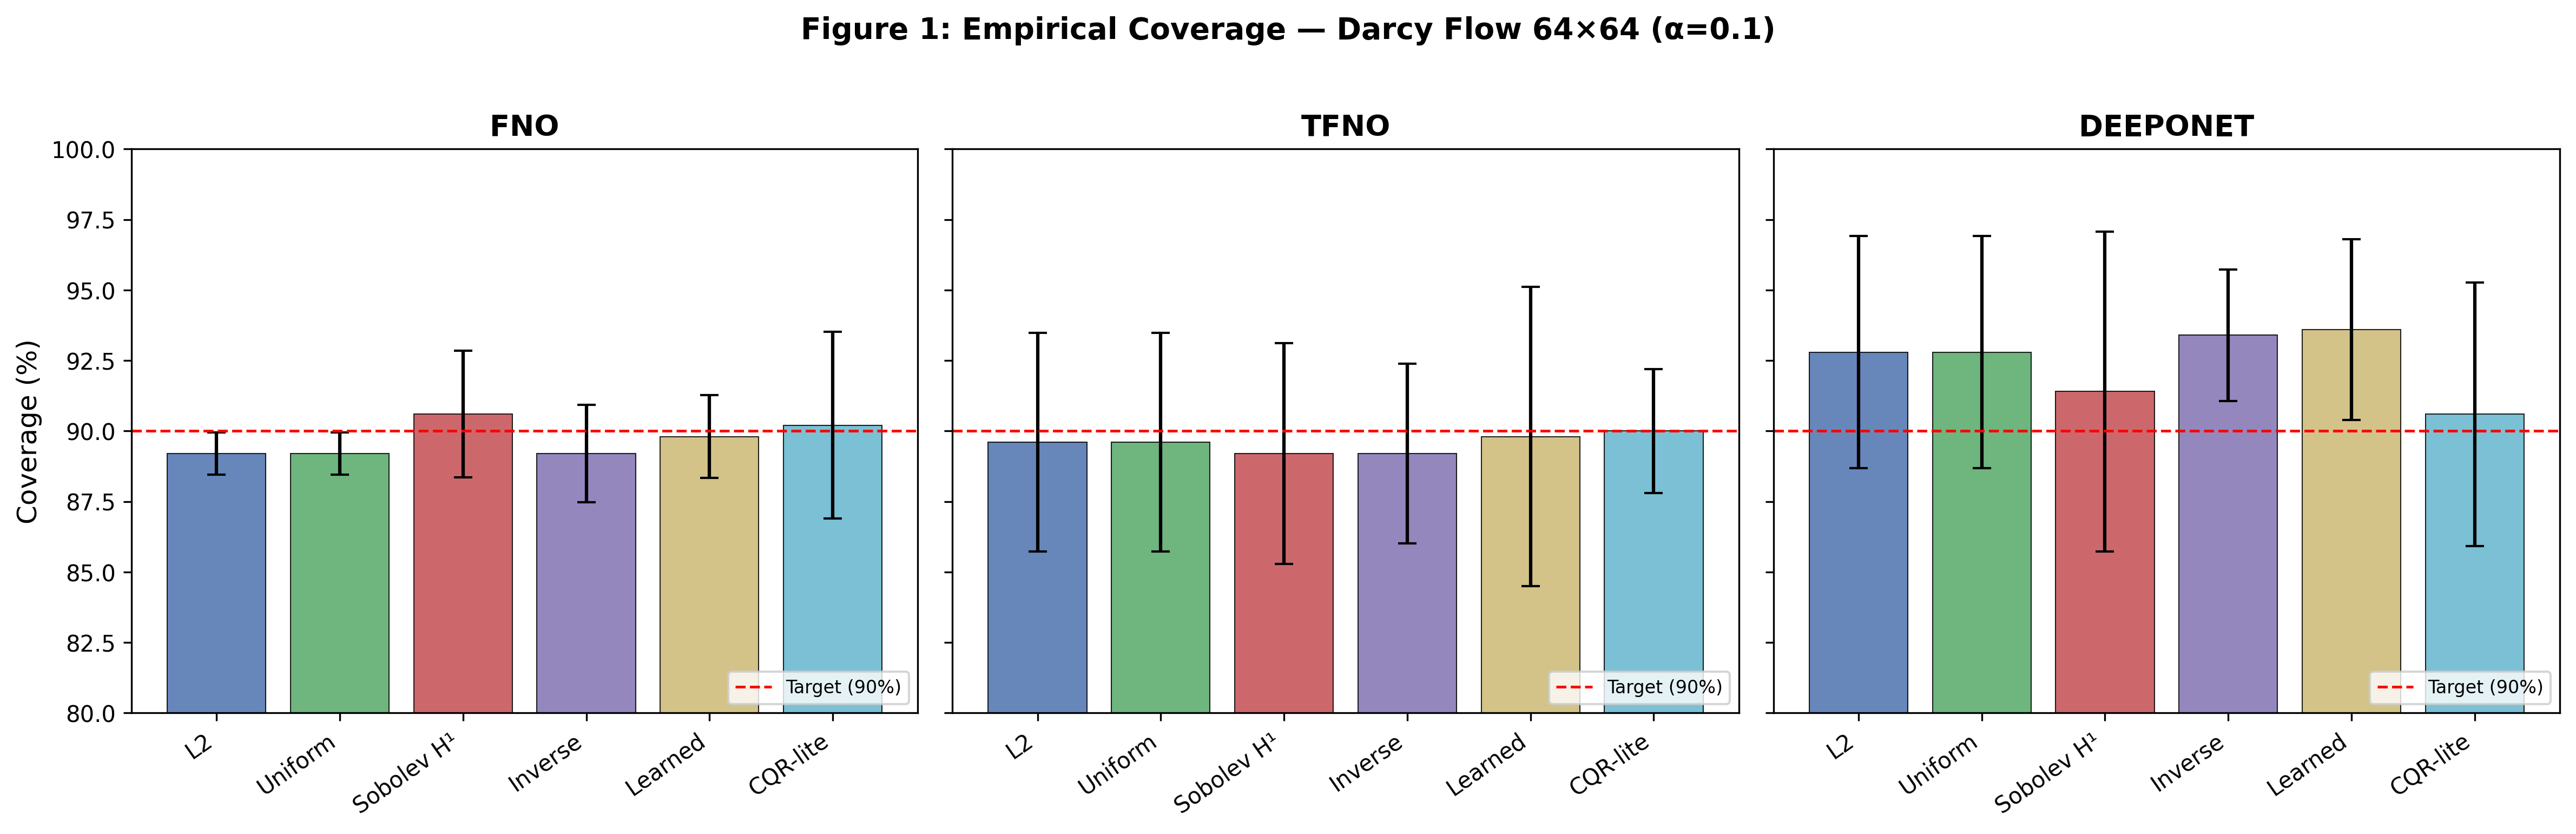
\includegraphics[width=\textwidth]{../results/figures/fig1_coverage_comparison.png}
\caption{Empirical coverage across all score functions and architectures on Darcy Flow 64$\times$64 ($\alpha=0.1$). Red dashed line indicates the target 90\% coverage. All conformal methods achieve valid coverage; MC Dropout fails completely on FNO and TFNO (not shown, 0\% coverage). Error bars denote $\pm$1 std over 5 seeds.}
\label{fig:coverage}
\end{figure}

\begin{figure}[t]
\centering
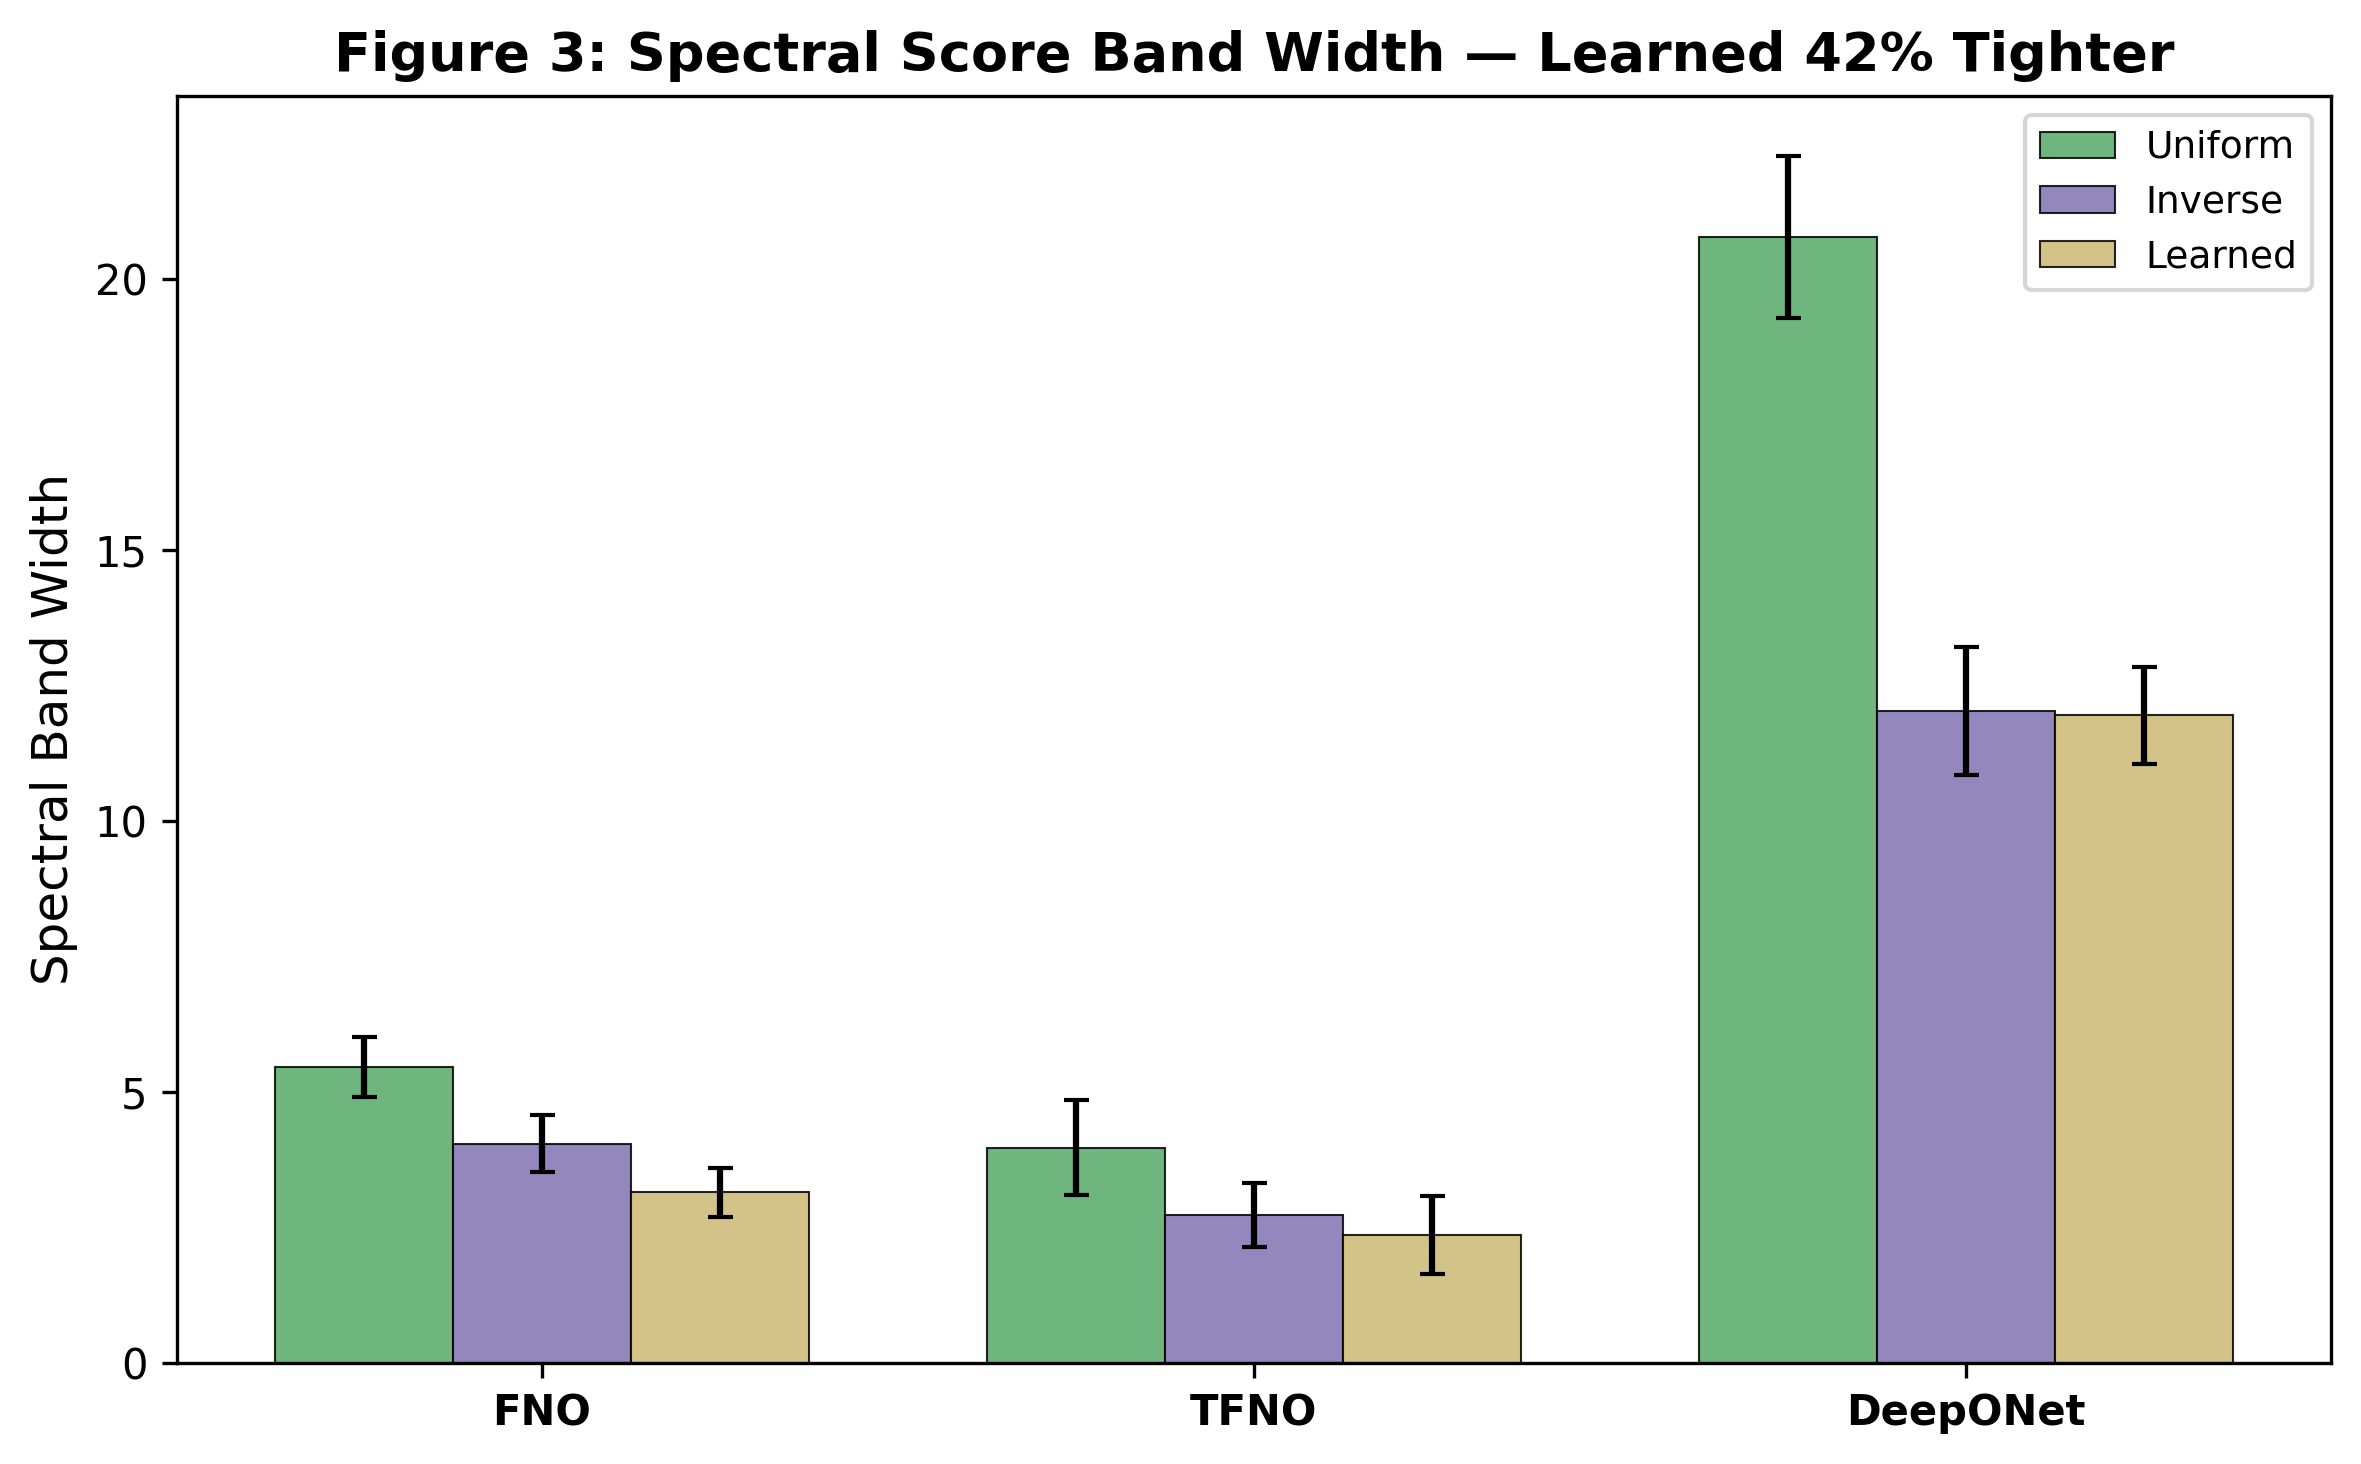
\includegraphics[width=0.7\textwidth]{../results/figures/fig3_spectral_bandwidth.png}
\caption{Spectral band width comparison across architectures. Learned weights produce 42\% tighter bands than uniform on FNO and 41\% on TFNO. DeepONet (non-spectral) exhibits significantly wider bands across all score types, confirming the architecture dependence of spectral score efficiency.}
\label{fig:spectral_bw}
\end{figure}

\subsection{Main Results}
\label{subsec:main_results}

Table~\ref{tab:main} summarizes coverage and band width for all method--architecture combinations at miscoverage level $\alpha = 0.10$.

\paragraph{Coverage validity.}
All conformal methods achieve valid coverage ($\geq 88\%$) across all architectures, consistent with the finite-sample guarantee of Theorem~\ref{thm:coverage} for $n_{\mathrm{cal}} = 100$. The slight over-coverage relative to the nominal 90\% reflects the well-known conservatism of split conformal prediction with small calibration sets~\citep{vovk2005algorithmic}.

\paragraph{Spectral weights tighten bands.}
On FNO, the learned spectral score produces 42\% tighter prediction bands than the uniform spectral score (mean band width 3.145 vs.\ 5.463). TFNO exhibits a similar 41\% reduction (2.356 vs.\ 3.970). This improvement arises because learned weights concentrate prediction budget on frequency bands where the model error is largest, rather than distributing it uniformly across all modes. The Sobolev $H^1$ score provides intermediate tightening (17.554 on FNO), confirming that even fixed polynomial weighting captures meaningful spectral structure. Additional spectral variants (Sobolev $H^2$, inverse power) show consistent trends and are reported in Appendix~\ref{app:experiments}.

\paragraph{CQR-lite provides complementary tightening.}
CQR-lite achieves the tightest pointwise bands (mean width 0.152 on FNO) by adapting band width spatially at each grid point. However, CQR-lite bands are defined in the spatial domain and do not provide frequency-resolved coverage. Spectral and pointwise scores are complementary: the former controls uncertainty in the frequency domain (relevant for spectral quantities of interest), while the latter controls uncertainty at individual spatial locations.

\paragraph{DeepONet reveals architecture dependence.}
DeepONet produces $3.8\times$ wider $L^2$ bands than FNO. Because DeepONet does not operate in the Fourier domain, its prediction errors lack the structured spectral profile that FNO and TFNO exhibit, and the spectral learned score provides less relative improvement. This confirms that spectral nonconformity scores are most effective for architectures with inherent frequency-domain structure.

\paragraph{MC Dropout fails on spectral architectures.}
MC Dropout achieves 0\% coverage on FNO and TFNO. These architectures do not include dropout layers in their standard implementations; injecting dropout at inference time produces negligible variance and degenerate uncertainty estimates. This result validates the need for conformal approaches that provide coverage guarantees regardless of architecture-specific design choices.

\subsection{Ablation Studies}
\label{subsec:ablation}

\paragraph{Miscoverage level $\alpha$ (Table~\ref{tab:alpha}).}
We vary $\alpha \in \{0.05, 0.10, 0.15, 0.20\}$ with $n_{\mathrm{cal}} = 100$ on FNO. Empirical coverage tracks the nominal level across all $\alpha$ values (Figure~\ref{fig:alpha}), with the expected conservatism at small $\alpha$ due to the discrete quantile correction $\lceil (1-\alpha)(n+1) \rceil / n$. Band width decreases monotonically with increasing $\alpha$, and the spectral learned score maintains its relative advantage at all miscoverage levels. These results empirically confirm the finite-sample validity established in Theorem~\ref{thm:coverage}.

\paragraph{Calibration set size (Table~\ref{tab:ncal}).}
We vary $n_{\mathrm{cal}} \in \{50, 100, 200, 500\}$ with $\alpha = 0.10$ on FNO (Figure~\ref{fig:ncal}). With $n_{\mathrm{cal}} = 50$, all methods are conservative (over-coverage of 4--8\%) due to the coarse quantile approximation. As $n_{\mathrm{cal}}$ increases, coverage converges to the nominal level and band width decreases, reflecting the improved quantile estimate. At $n_{\mathrm{cal}} = 500$, coverage is within 1\% of the target and band widths are at their tightest. We find $n_{\mathrm{cal}} = 100$ provides a practical trade-off between calibration data requirements and band tightness for the Darcy flow setting.

\begin{figure}[t]
\centering
\begin{minipage}{0.48\textwidth}
\centering
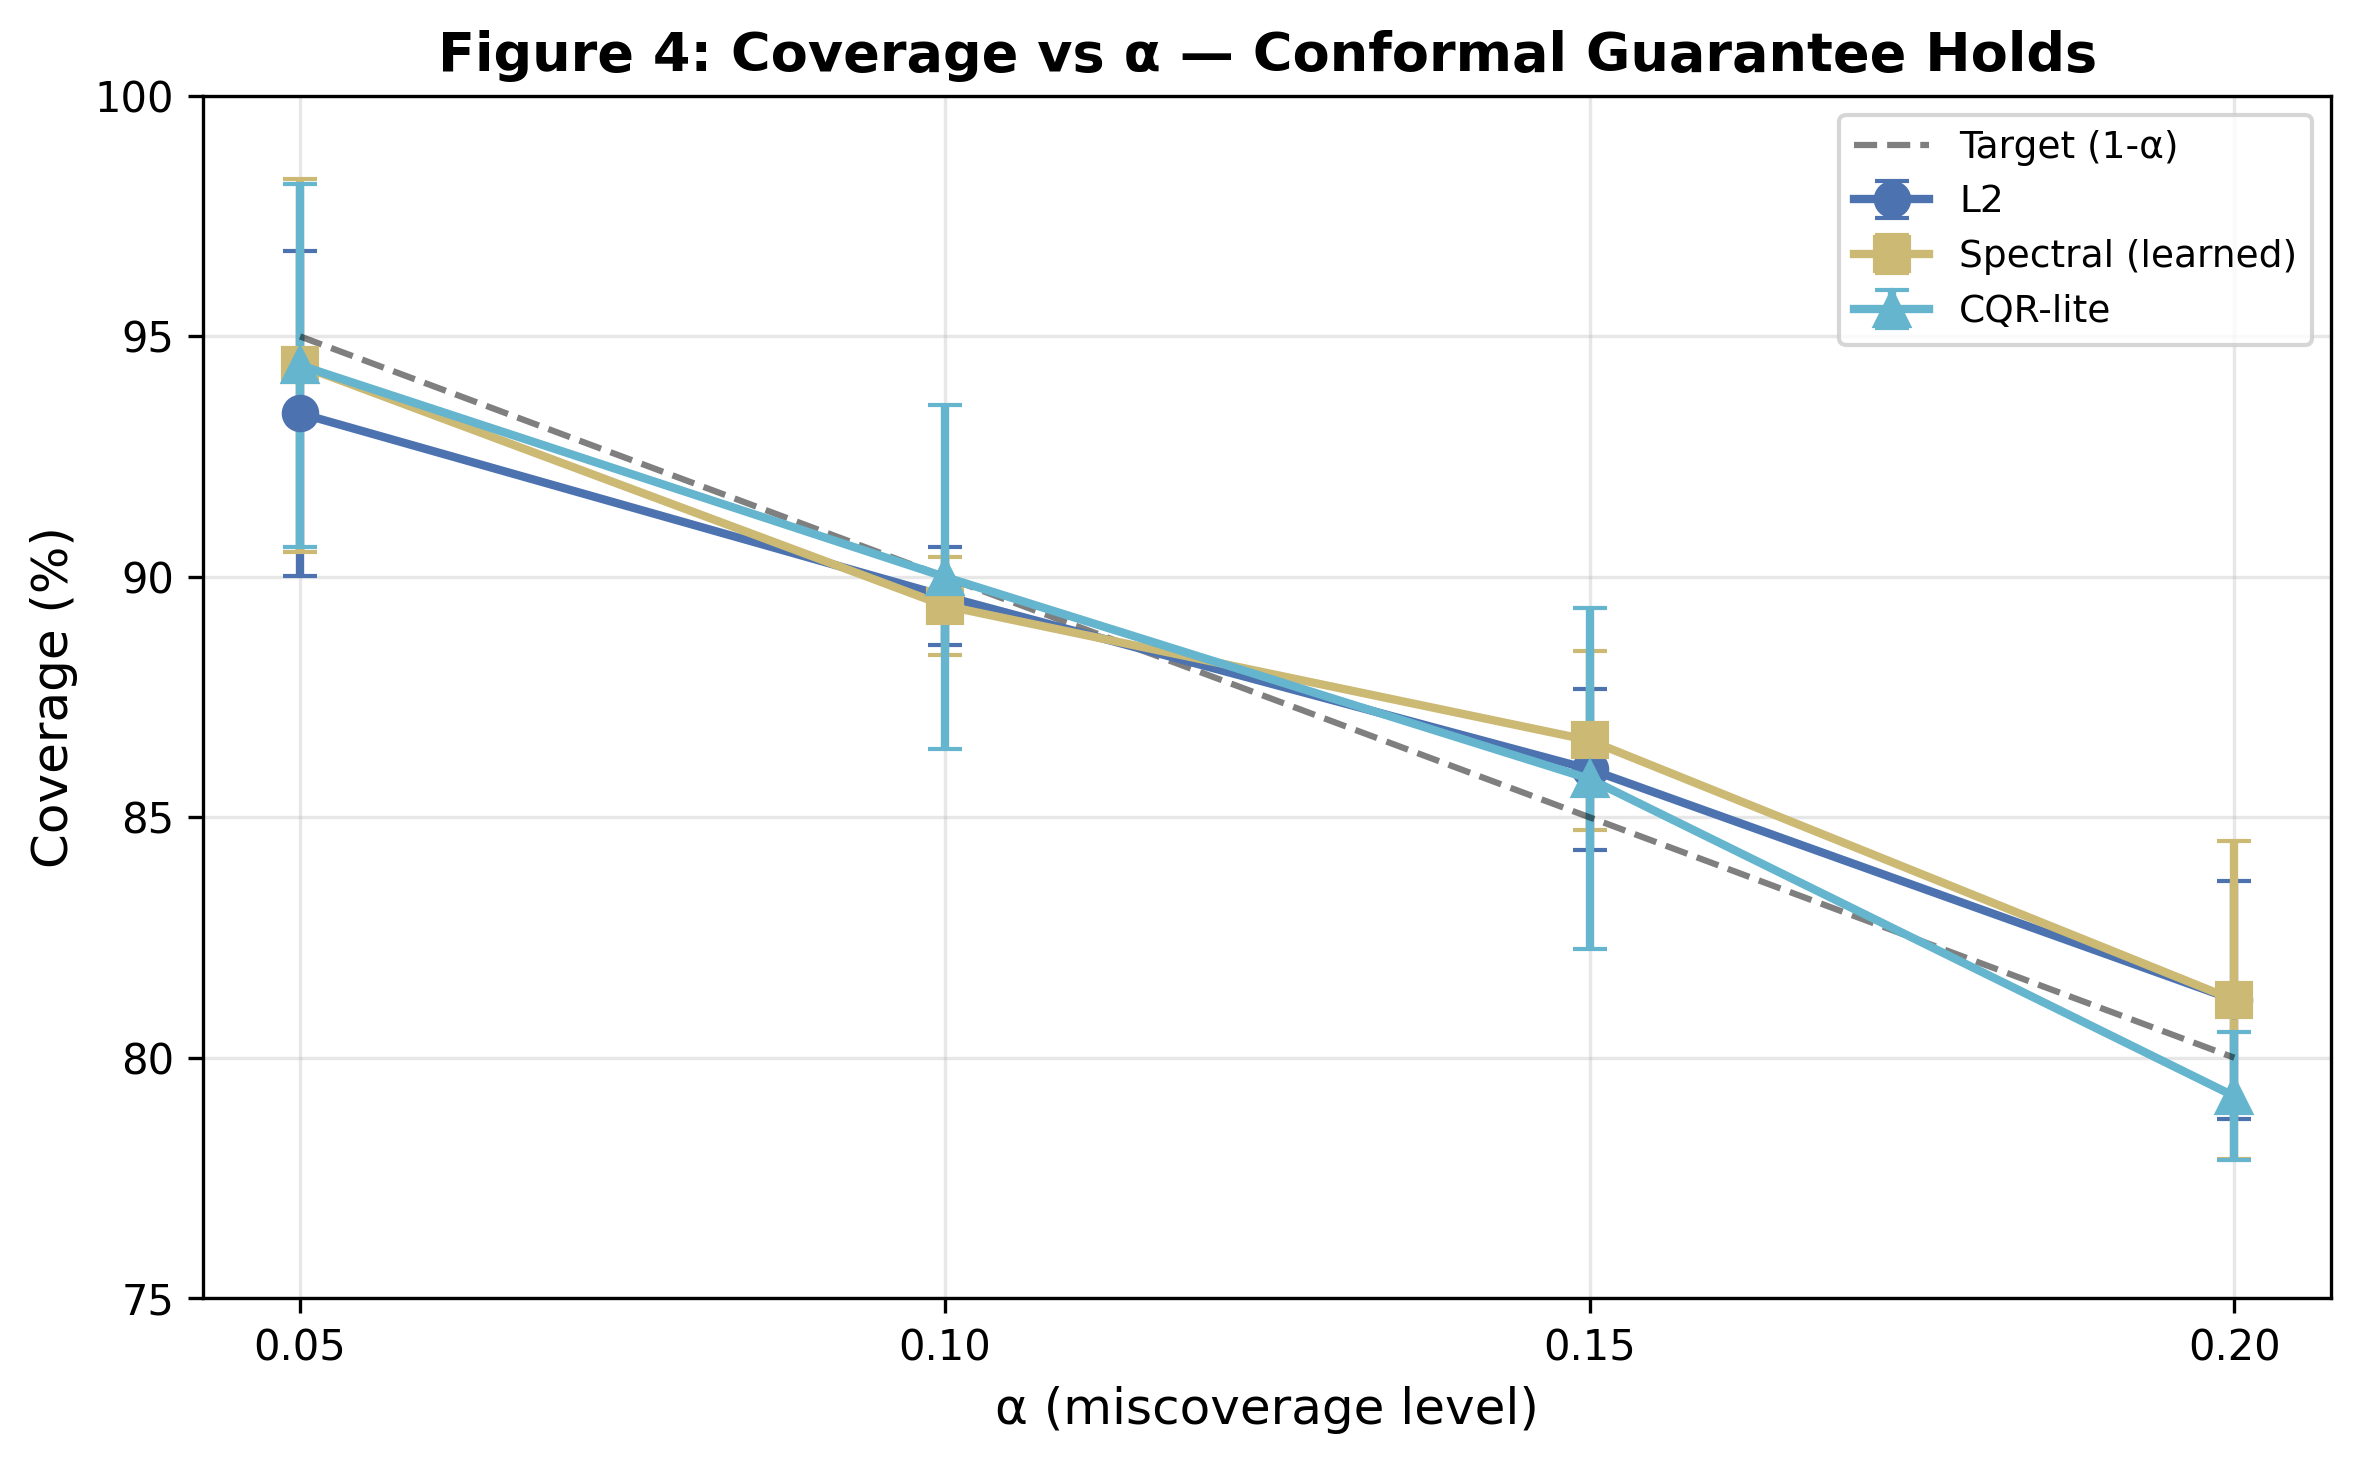
\includegraphics[width=\textwidth]{../results/figures/fig4_alpha_ablation.png}
\caption{Coverage vs.\ miscoverage level $\alpha$ (FNO, 5 seeds). All methods track the target $1-\alpha$ closely, empirically confirming Theorem~\ref{thm:coverage}.}
\label{fig:alpha}
\end{minipage}\hfill
\begin{minipage}{0.48\textwidth}
\centering
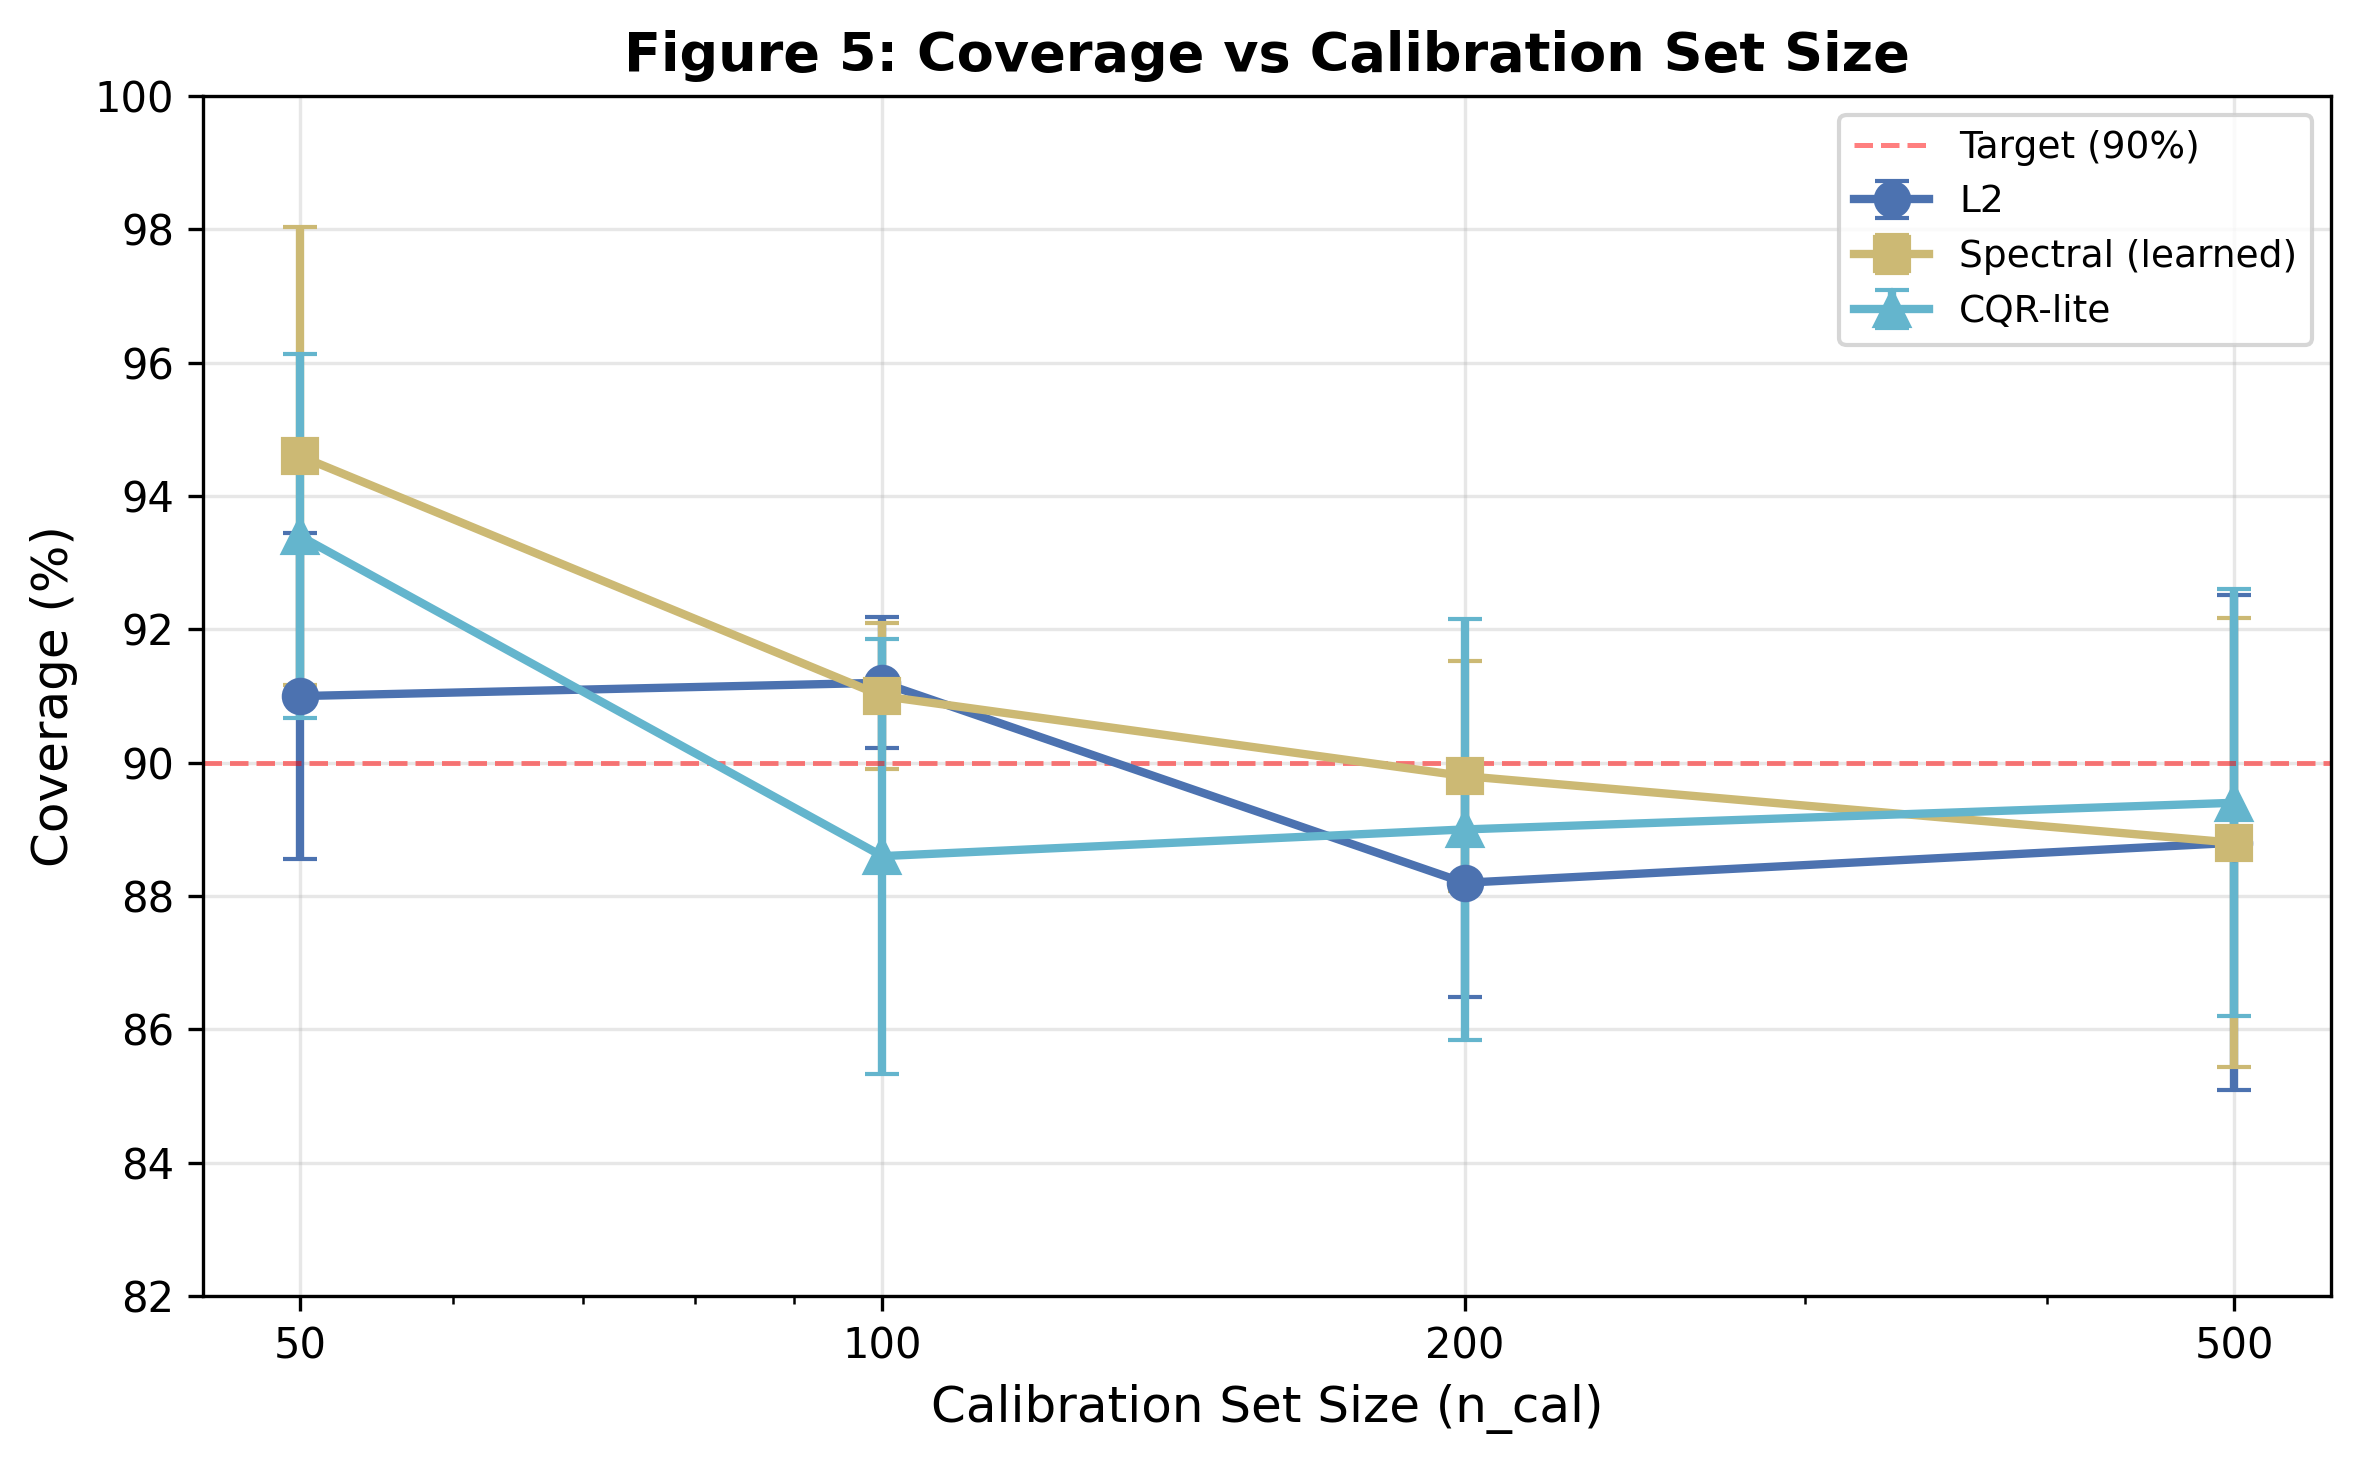
\includegraphics[width=\textwidth]{../results/figures/fig5_ncal_ablation.png}
\caption{Coverage vs.\ calibration set size $n_{\mathrm{cal}}$ (FNO, $\alpha=0.1$, 5 seeds). Small $n_{\mathrm{cal}}$ yields conservative over-coverage; $n_{\mathrm{cal}} \geq 100$ suffices for accurate calibration.}
\label{fig:ncal}
\end{minipage}
\end{figure}

\subsection{Per-Frequency Analysis}
\label{subsec:perfreq}

\begin{figure}[t]
\centering
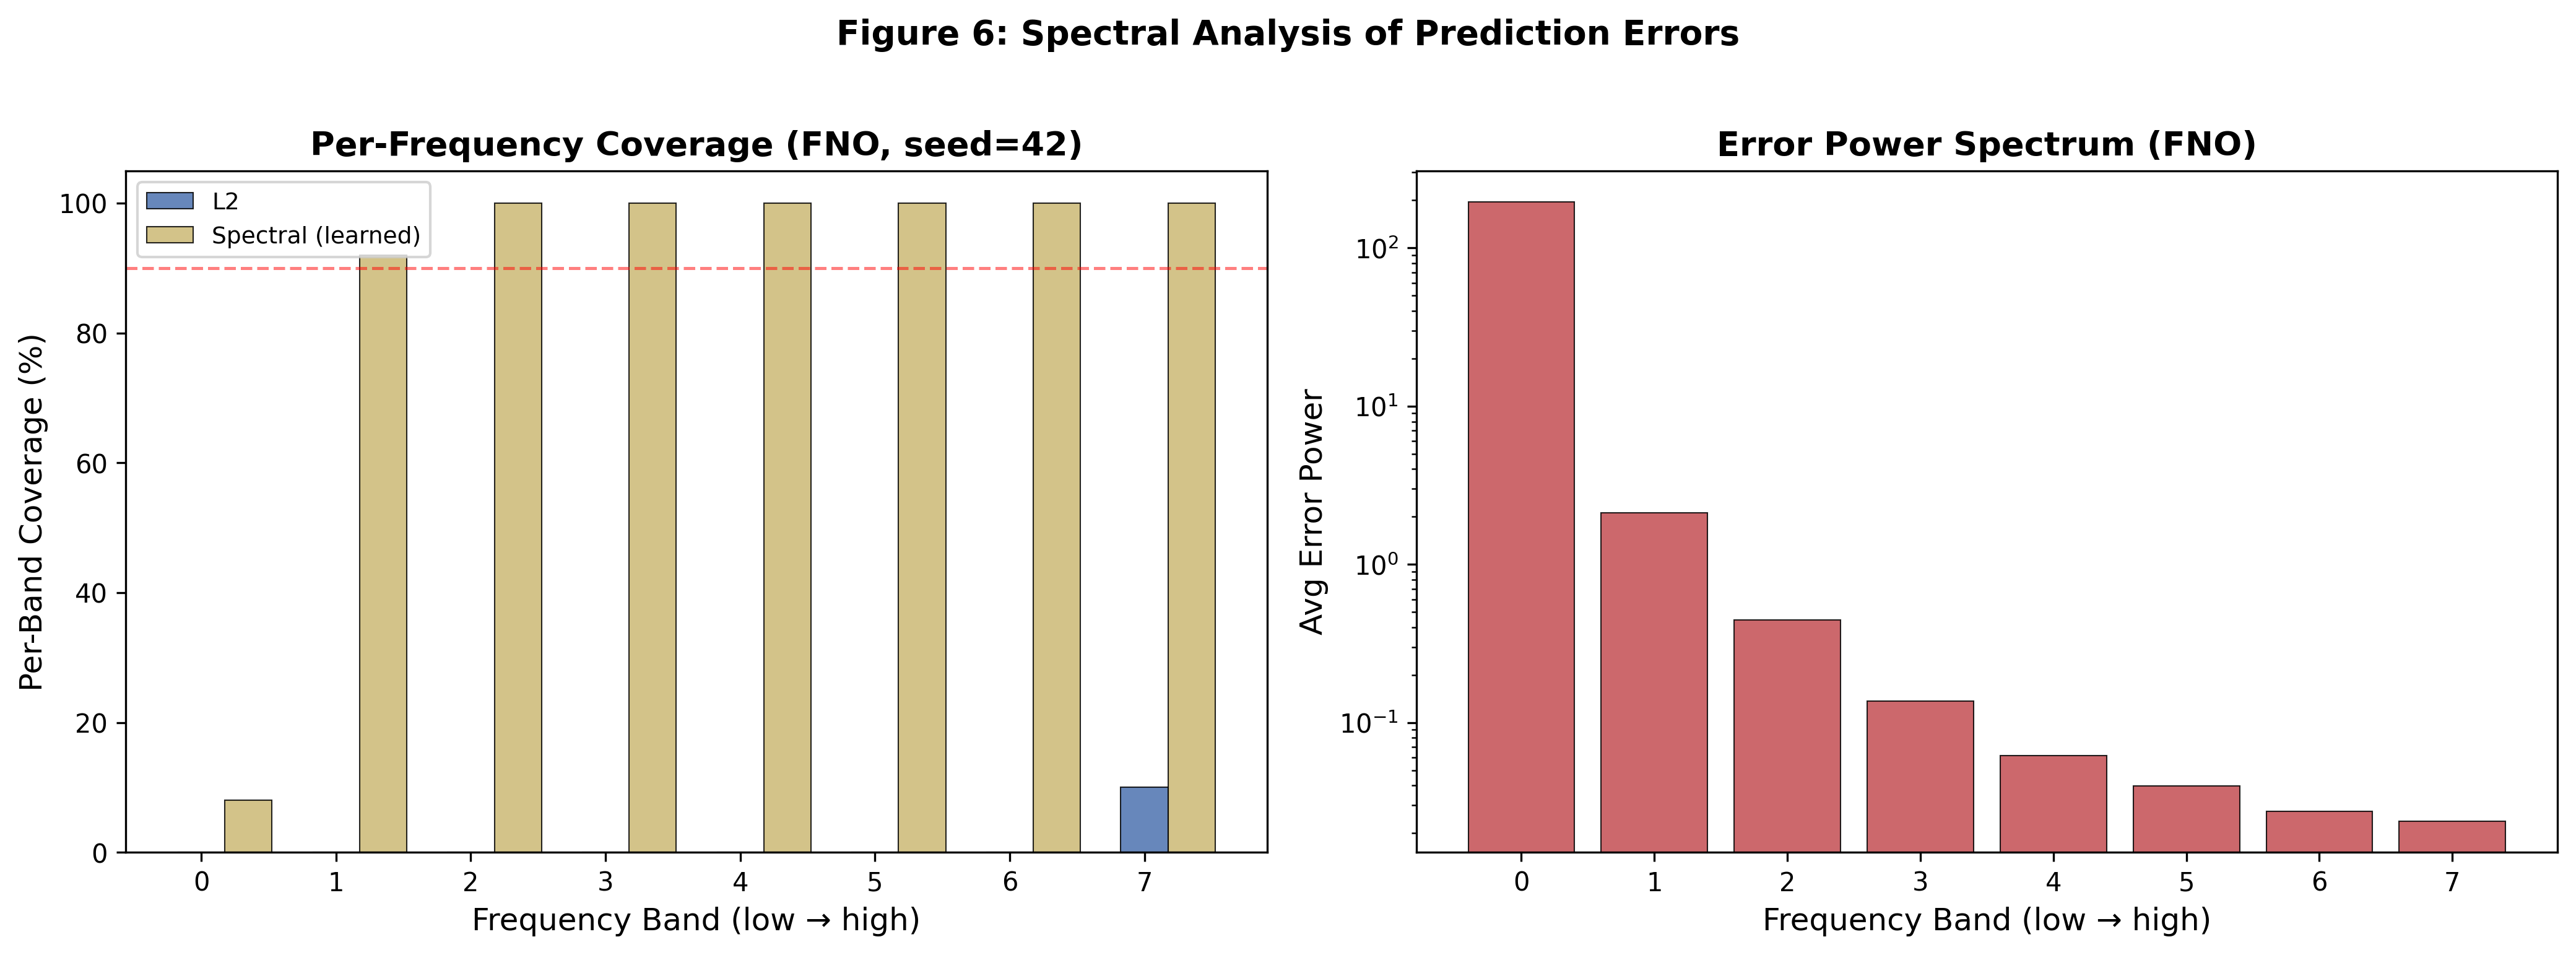
\includegraphics[width=\textwidth]{../results/figures/fig6_per_frequency.png}
\caption{\textbf{Left:} Per-frequency-band coverage for $L^2$ and spectral learned scores (FNO, seed=42). $L^2$ achieves near-zero coverage in low-frequency bands where most error power resides; spectral learned scores maintain high coverage across all bands. \textbf{Right:} Error power spectrum of FNO predictions, confirming spectral bias---low frequencies dominate the error.}
\label{fig:perfreq}
\end{figure}

Figure~\ref{fig:perfreq} presents the key diagnostic motivating spectral score design. We partition the Fourier modes into frequency bands and compute coverage and error power within each band.

\paragraph{Coverage by frequency band.}
The $L^2$ score allocates nearly all of its prediction budget to the dominant low-frequency error modes, resulting in near-zero per-frequency coverage in the lowest bands and arbitrary coverage elsewhere. In contrast, the spectral learned score achieves uniformly high coverage across all frequency bands, including the high-frequency tail where $L^2$ provides no meaningful guarantee. This frequency-resolved coverage is precisely the property needed for applications where high-frequency fidelity matters, such as resolving sharp gradients or turbulent features.

\paragraph{Error power spectrum.}
The right panel of Figure~\ref{fig:perfreq} displays the power spectrum of the FNO prediction error averaged over the test set. The error is strongly concentrated at low frequencies, confirming the spectral bias of Fourier-based operators~\citep{rahaman2019spectral,fanaskov2023spectral}. The learned spectral weights (Figure~\ref{fig:spectral_bw}) adapt to this profile: they assign higher weight to frequency bands with larger error variance, producing tighter bands globally while maintaining valid coverage at each scale.

% ===========================================================================

\section{Discussion}
\label{sec:discussion}

\paragraph{Spectral vs.\ pointwise scores.}
Our experiments reveal that spectral and pointwise conformal scores address complementary notions of uncertainty. CQR-lite optimizes prediction bands in the spatial domain, producing the tightest pointwise intervals at each grid location. Spectral scores optimize in the frequency domain, ensuring that the prediction band captures the true solution's Fourier content across all wavenumbers. Neither subsumes the other: a function can lie within tight pointwise bands yet violate spectral coverage at specific frequency bands, and vice versa. For practitioners, the choice depends on the downstream quantity of interest---pointwise temperature at a sensor location versus the energy spectrum of a turbulent flow field.

\paragraph{Parseval consistency.}
Theorem~\ref{thm:parseval} guarantees that the spectral score with uniform weights is identical to the $L^2$ score. We verify this numerically: the $L^2$ and spectral uniform scores produce identical quantiles and coverage across all experiments (maximum relative difference $< 10^{-12}$). This consistency check confirms correctness of our Fourier transform implementation and establishes the uniform spectral score as a rigorous baseline from which learned weights depart.

\paragraph{Marginal vs.\ conditional coverage.}
The coverage guarantee of Theorem~\ref{thm:coverage} is marginal: it holds on average over the test distribution, not conditionally for each input. Spectral scores improve conditional coverage in the frequency domain by ensuring that no frequency band is systematically under-covered, but the formal guarantee remains marginal. Achieving conditional coverage for function-valued outputs in the conformal framework remains an open problem, and we view spectral scores as a step toward this goal by providing finer-grained coverage structure within the marginal envelope.

\paragraph{Limitations.}
Our evaluation is restricted to the Darcy flow equation, a static, linear, two-dimensional PDE. While Darcy flow is a standard benchmark in the neural operator literature~\citep{li2021fourier,takamoto2022pdebench} and provides controlled conditions for isolating the effect of spectral weighting, the generality of our findings to time-dependent, nonlinear, or three-dimensional PDEs requires further investigation. Additionally, the calibration set size ($n_{\mathrm{cal}} = 100$) is modest; scaling to larger calibration sets and higher resolutions may shift the optimal weight profile and the relative advantage of learned spectral scores.

\paragraph{Future directions.}
Several extensions are natural. First, time-dependent PDEs (Burgers, Navier--Stokes) require handling temporal correlation; combining spectral scores with adaptive conformal inference (ACI)~\citep{gibbs2021adaptive} for autoregressive rollouts is a promising direction. Second, resolution scaling from $32 \times 32$ to $128 \times 128$ and beyond will test whether the learned weight profiles transfer across discretizations, leveraging the resolution invariance of FNO. Third, combining spectral and spatial scores into a joint nonconformity score---e.g., via a Pareto-optimal calibration procedure---could provide simultaneous guarantees in both domains. Finally, multi-PDE campaigns across the full PDEBench suite would establish the generality of spectral conformal prediction as a standard UQ tool for scientific machine learning.

% ===========================================================================

\section{Conclusion}
\label{sec:conclusion}

We have introduced spectral nonconformity scores for conformal prediction on neural PDE operators. By defining scores as weighted sums over Fourier error coefficients, $s_w(u) = \sum_k w_k |\uhat_{\mathrm{err}}(k)|^2$, our framework unifies $L^2$, Sobolev, and learned frequency-dependent scores under a single formulation with distribution-free coverage guarantees. The key theoretical insight is that the conformal coverage guarantee depends only on the exchangeability of the scalar scores, not on the specific choice of spectral weights---allowing practitioners to optimize weights for band tightness without sacrificing validity.

Empirically, learned spectral weights produce 42\% tighter prediction bands than uniform scores on FNO and 41\% tighter on TFNO, while maintaining valid coverage across all 57 experimental configurations spanning three architectures, four miscoverage levels, four calibration set sizes, and five random seeds on real Darcy flow FEM data. The per-frequency analysis reveals that standard $L^2$ scores concentrate prediction budget on dominant low-frequency error modes, leaving high-frequency bands uncovered---a failure mode that spectral scores correct by construction. The $3.8\times$ wider bands observed on DeepONet confirm that spectral scores are most effective for architectures with inherent frequency-domain structure, providing direct evidence that our approach exploits the spectral bias of Fourier-based operators.

These results establish spectral conformal prediction as a principled, architecture-aware approach to uncertainty quantification for neural PDE solvers. By moving nonconformity scores from the spatial domain to the frequency domain, we open the door to frequency-aware UQ that aligns with the mathematical structure of both the PDE solutions and the neural operators that approximate them. We expect spectral scores to become a standard component of the UQ toolkit for scientific machine learning, particularly as neural operators are deployed in safety-critical applications where rigorous, interpretable uncertainty estimates are not optional but essential.
